\documentclass[aspectratio=169, 10pt]{beamer}

% --- PACKAGES ---
\usepackage[utf8]{inputenc}
\usepackage[T1]{fontenc}
\usepackage{helvet}
\usepackage{booktabs}
\usepackage{xcolor}
\usepackage{tcolorbox}
\usepackage{graphicx}
\usepackage{tabularx}
\usepackage{adjustbox}

% --- VISUAL THEME ---
\usetheme{default}
\usecolortheme{default}

\definecolor{BBPBlue}{HTML}{2C3E50}
\definecolor{BBPAccent}{HTML}{27AE60}
\definecolor{BBPGray}{HTML}{95A5A6}
\definecolor{BBPAlert}{HTML}{E74C3C}
\definecolor{BBPLight}{HTML}{ECF0F1}

% Font settings
\setbeamerfont{title}{series=\bfseries, size=\huge}
\setbeamerfont{frametitle}{series=\bfseries, size=\Large}
\setbeamerfont{block title}{series=\bfseries}

% Color assignments
\setbeamercolor{title}{fg=BBPBlue}
\setbeamercolor{frametitle}{fg=BBPBlue}
\setbeamercolor{structure}{fg=BBPBlue}
\setbeamercolor{alerted text}{fg=BBPAlert}
\setbeamercolor{block title}{bg=BBPBlue, fg=white}
\setbeamercolor{block body}{bg=BBPLight, fg=black}

% Clean layout
\setbeamertemplate{navigation symbols}{}
\setbeamertemplate{itemize items}[circle]
\setbeamertemplate{enumerate items}[default]

\setbeamertemplate{footline}{
    \hfill\color{BBPGray}\scriptsize \insertframenumber\hspace{1em}\vspace{1em}
}

% --- METADATA ---
\title{Best Bike Paths (BBP)}
\subtitle{Requirements Analysis \& Design Presentation}
\author{Software Engineering II Project}
\institute{Politecnico di Milano}
\date{A.Y. 2025-2026}

\begin{document}

% =========================================================
% TITLE
% =========================================================
\begin{frame}[plain]
    \vspace{1cm}
    \maketitle
\end{frame}

% =========================================================
% PART 1: RASD
% =========================================================
\section{RASD: Requirements Analysis}

% SLIDE 1: Goals
\begin{frame}{1. System Goals}
    \textbf{What BBP aims to achieve:}
    
    \vspace{0.3cm}
    \begin{block}{Primary Objectives}
        \begin{itemize}
            \item \textbf{G02}: Enable cyclists to record personal trips (Manual/Automatic)
            \item \textbf{G06}: Provide human-in-the-loop validation of sensor data
            \item \textbf{G13}: Compute safety scores for bike paths
            \item \textbf{G15}: Detect road anomalies using mobile sensors
            \item \textbf{G16}: Merge multiple user contributions intelligently
            \item \textbf{G09}: Offer community access to safety information
        \end{itemize}
    \end{block}
    
    \vspace{0.2cm}
    \textbf{Core Value:} Transform individual cycling experiences into collective safety intelligence.
\end{frame}

% SLIDE 2: Boundaries
\begin{frame}{2. System Boundaries}
    \textbf{World vs. Machine Phenomena:}
    
    \vspace{0.3cm}
    \begin{columns}[T]
        \column{0.48\textwidth}
        \begin{block}{World-Controlled (Real World)}
            \begin{itemize}
                \item \textbf{WP01}: Users bike through streets
                \item \textbf{WP03}: Obstacles occur (potholes, debris)
                \item \textbf{WP05}: Meteorological conditions exist
                \item \textbf{WP04}: Mobile sensors detect movement
            \end{itemize}
        \end{block}
        
        \column{0.48\textwidth}
        \begin{block}{Machine-Controlled (BBP System)}
            \begin{itemize}
                \item \textbf{SP06}: Infer anomalies from sensor data
                \item \textbf{SP10}: Display scored paths on map
                \item \textbf{SP12}: Merge path information from users
                \item \textbf{SP02}: Compute trip statistics
            \end{itemize}
        \end{block}
    \end{columns}
    
    \vspace{0.2cm}
    \textbf{Boundary:} BBP processes real-world phenomena but doesn't control physical streets.
\end{frame}

% SLIDE 3: Meaningful Use Case
\begin{frame}{3. Meaningful Use Case}
    \textbf{Scenario: Emma's Daily Commute}
    
    \vspace{0.3cm}
    \begin{enumerate}
        \item \textbf{Recording:} Emma starts automatic recording on her smartphone
        \item \textbf{Detection:} BBP identifies potholes via accelerometer spikes
        \item \textbf{Validation:} Post-ride, Emma confirms/rejects each detection
        \item \textbf{Publication:} She publishes the trip as "River Path - Morning"
        \item \textbf{Merging:} System combines her data with other cyclists' reports
        \item \textbf{Community Benefit:} Path appears in searches with score 8.5/10
    \end{enumerate}
    
    \vspace{0.3cm}
    \begin{block}{Key Elements}
        \begin{itemize}
            \item Sensor-based data acquisition
            \item Human validation step
            \item Community data merging
            \item Public safety benefit
        \end{itemize}
    \end{block}
\end{frame}

% SLIDE 4: Key Requirements
\begin{frame}{4. Most Important Requirements}
    \textbf{Critical Functional Requirements:}
    
    \vspace{0.3cm}
    \begin{columns}[T]
        \column{0.48\textwidth}
        \begin{block}{Data Acquisition}
            \begin{itemize}
                \item \textbf{R05}: Record GPS coordinates at intervals
                \item \textbf{R06}: Generate TrackPoint sequences
                \item \textbf{R09}: Enrich with weather data
                \item \textbf{R33}: Handle sensor unavailability
            \end{itemize}
        \end{block}
        
        \column{0.48\textwidth}
        \begin{block}{Safety Intelligence}
            \begin{itemize}
                \item \textbf{R15}: Link confirmed obstacles to streets
                \item \textbf{R24}: Update path scores based on reports
                \item \textbf{R31}: Retrieve external weather data
                \item \textbf{R16}: Respect publishability preferences
            \end{itemize}
        \end{block}
    \end{columns}
    
    \vspace{0.3cm}
    \textbf{Why these matter:} They enable reliable data collection and community safety intelligence.
\end{frame}

% SLIDE 5: Key Assumptions
\begin{frame}{5. Critical Assumptions \& Constraints}
    \begin{columns}[T]
        \column{0.48\textwidth}
        \textbf{Key Assumptions:}
        \begin{itemize}
            \item \textbf{A01}: Users have smartphones with required sensors
            \item \textbf{A04}: Stable internet for data synchronization
            \item \textbf{A05}: Users provide truthful information
            \item \textbf{A07}: Device clocks are correctly set
            \item \textbf{A06}: External services provide accurate data
        \end{itemize}
        
        \column{0.48\textwidth}
        \textbf{Design Constraints:}
        \begin{itemize}
            \item \textbf{C01}: GDPR compliance for location data
            \item \textbf{C05}: Functionality with intermittent connectivity
            \item \textbf{C06}: Battery consumption optimization
            \item \textbf{C02}: Support for heterogeneous devices
            \item \textbf{C04}: Only validated data shown to community
        \end{itemize}
    \end{columns}
    
    \vspace{0.3cm}
    \begin{alertblock}{Impact}
        These shape technical decisions: offline storage, privacy zones, sensor optimization.
    \end{alertblock}
\end{frame}

% SLIDE 6: Alloy Analysis
\begin{frame}{6. Formal Analysis with Alloy}
    \textbf{What we aim to prove:}
    
    \vspace{0.3cm}
    \begin{block}{Key Properties Verified}
        \begin{enumerate}
            \item \textbf{Trip Coherence:} Track points are temporally ordered
            \item \textbf{Obstacle Workflow:} Only CONFIRMED reports link to physical obstacles
            \item \textbf{Majority Voting:} Path status determined by most frequent reports
            \item \textbf{Data Consistency:} Manual trips have no track points, automatic trips do
        \end{enumerate}
    \end{block}
    
    \vspace{0.3cm}
    \begin{block}{Verification Results}
        \begin{itemize}
            \item \texttt{confirmedMeansObstacle}: Verified - no counterexamples
            \item \texttt{bikePathStatusIsMajority}: Verified - majority rule holds
            \item \texttt{tripTimesAreConsistent}: Verified - temporal constraints satisfied
        \end{itemize}
    \end{block}
    
    \vspace{0.2cm}
    \textbf{Value:} Formal assurance of critical business logic correctness.
\end{frame}

% =========================================================
% PART 2: DD
% =========================================================
\section{DD: Design Document}

% SLIDE 7: Components
\begin{frame}{7. System Components}
    \textbf{Microservices Architecture:}
    
    \vspace{0.3cm}
    \begin{columns}[T]
        \column{0.32\textwidth}
        \begin{block}{Client Layer}
            \begin{itemize}
                \item Mobile Application
                \item UI Controller
                \item Sensor Manager
                \item Local DB Manager
            \end{itemize}
        \end{block}
        
        \column{0.32\textwidth}
        \begin{block}{Backend Services}
            \begin{itemize}
                \item Trip Ingestion Service
                \item Validation Service
                \item Aggregation Service
                \item Scoring Service
            \end{itemize}
        \end{block}
        
        \column{0.32\textwidth}
        \begin{block}{Specialized Servers}
            \begin{itemize}
                \item Trip Search Server
                \item Report Server
                \item Users Account Manager
            \end{itemize}
        \end{block}
    \end{columns}
    
    \vspace{0.3cm}
    \begin{block}{Data Layer (Polyglot Persistence)}
        \begin{itemize}
            \item User Data (PostgreSQL)
            \item Trips Data (Time-series DB)
            \item Score Data (PostGIS)
            \item Reports Data (PostgreSQL)
        \end{itemize}
    \end{block}
\end{frame}

% SLIDE 8: Interfaces
\begin{frame}{8. Component Interfaces}
    \textbf{Key API Contracts:}
    
    \vspace{0.3cm}
    \begin{columns}[T]
        \column{0.48\textwidth}
        \begin{block}{Client-Facing (IBBPClientAPI)}
            \begin{itemize}
                \item \texttt{POST /v1/trips/upload}
                \item \texttt{GET /v1/trips/search}
                \item \texttt{POST /v1/reports/obstacle}
                \item \texttt{PUT /v1/trips/{id}/publish}
            \end{itemize}
        \end{block}
        
        \column{0.48\textwidth}
        \begin{block}{Internal Services}
            \begin{itemize}
                \item \texttt{ITripCompliance} (Validation)
                \item \texttt{ITripAggregation} (Merging)
                \item \texttt{IScoringCalculation} (Scoring)
                \item \texttt{IReportManagement} (Reports)
            \end{itemize}
        \end{block}
    \end{columns}
    
    \vspace{0.3cm}
    \begin{block}{External Adapters}
        \begin{itemize}
            \item \texttt{IMeteoProvider}: Weather API wrapper
            \item \texttt{IMapProvider}: OpenStreetMap integration
        \end{itemize}
    \end{block}
    
    \vspace{0.2cm}
    \textbf{Design:} Clear separation with DTOs for type safety.
\end{frame}
% SLIDE 9a: Architectural Patterns
\begin{frame}{9a. Architectural Styles \& Patterns}
    \begin{columns}[T]
        \column{0.48\textwidth}
        \begin{block}{Microservices Architecture}
            \textbf{Why:} Independent scalability, fault isolation
            \begin{itemize}
                \item Each service deployable independently
                \item Technology heterogeneity allowed
                \item Clear bounded contexts
            \end{itemize}
        \end{block}
        
        \begin{block}{API Gateway Pattern}
            \textbf{Why:} Single entry point, cross-cutting concerns
            \begin{itemize}
                \item Request routing
                \item Authentication/SSL termination
                \item Rate limiting
            \end{itemize}
        \end{block}
      
        
        \column{0.48\textwidth}
        \begin{block}{CQRS Pattern}
            \textbf{Why:} Optimize read vs. write performance
            \begin{itemize}
                \item Write side: Trip ingestion pipeline
                \item Read side: Dedicated search server
                \item Prevents resource contention
            \end{itemize}
        \end{block}
        
    \end{columns}
\end{frame}

% SLIDE 9b: Architectural Patterns
\begin{frame}{9b. Architectural Styles \& Patterns}
    \begin{columns}[T]
        \column{0.48\textwidth}
        
        
        \begin{block}{Containerization \& Orchestration}
            \textbf{Technology:} \textbf{Kubernetes} (as per DD Chapter 2.3)
            \begin{itemize}
                \item Containerized microservices
                \item Automated scaling during peak hours
                \item Self-healing with health checks
                \item Service discovery \& load balancing
            \end{itemize}
        \end{block}
        
        \column{0.48\textwidth}

        \begin{block}{Polyglot Persistence}
            \textbf{Why:} Right tool for each data type
            \begin{itemize}
                \item Time-series for sensor logs
                \item PostGIS for geospatial queries
                \item Relational for user data
            \end{itemize}
        \end{block}
        
        \begin{block}{Deployment Infrastructure}
            \begin{itemize}
                \item Kubernetes cluster with Ingress Controller
                \item Secrets \& ConfigMaps for secure configuration
                \item Cloud infrastructure (AWS RDS, Timestream)
            \end{itemize}
        \end{block}
    \end{columns}
\end{frame}

% SLIDE 10: Meaningful Interactions
\begin{frame}{10. Meaningful Interactions}
    \textbf{Trip Processing Pipeline:}
    
    \vspace{0.3cm}
    \begin{enumerate}
        \item \textbf{Recording:} Mobile App → Sensor Manager → Local DB
        \item \textbf{Upload:} Network Manager → API Gateway → Trip Ingestion
        \item \textbf{Validation:} Ingestion → Validation Service → Map Matching
        \item \textbf{Aggregation:} Validation → Aggregation Service → Voting Engine
        \item \textbf{Scoring:} Aggregation → Scoring Service → Score update
        \item \textbf{Search:} User → Search Server → Spatial queries → Results
    \end{enumerate}
    
    \vspace{0.3cm}
    \begin{block}{Key Interaction Patterns}
        \begin{itemize}
            \item \textbf{Asynchronous Processing:} HTTP 202 responses for background jobs
            \item \textbf{Eventual Consistency:} Scores updated after processing
            \item \textbf{Human-in-the-loop:} Validation before obstacle confirmation
            \item \textbf{Offline Resilience:} Local buffering during connectivity loss
        \end{itemize}
    \end{block}
\end{frame}
% SLIDE 11: UI Mockups
\begin{frame}{11a. User Interface Design}
    \textbf{Mobile-First Approach for Cyclists}
    
    \vspace{0.3cm}
    \begin{columns}[T]
        \column{0.48\textwidth}
        \begin{block}{Auto Recording Interface}
            \begin{itemize}
                \item Real-time metrics display
                \item Weather conditions integration
                \item Simple start/stop controls
                \item Designed for safe cycling interaction
            \end{itemize}
        \end{block}
        
        \vspace{0.3cm}
    
        \column{0.48\textwidth}
        \begin{block}{Trip Search Interface}
            \begin{itemize}
                \item Color-coded paths by safety score
                \item Filtering by score/conditions
                \item Obstacle visualization on map
                \item Accessible to unregistered users
            \end{itemize}
        \end{block}
        \vspace{0.3cm}
    \end{columns}
\end{frame}
% SLIDE 11b: UI Mockups (Compact)
\begin{frame}{11b. User Interface Design}
    \centering
    \begin{columns}[c]
        \column{0.33\textwidth}
        \centering
        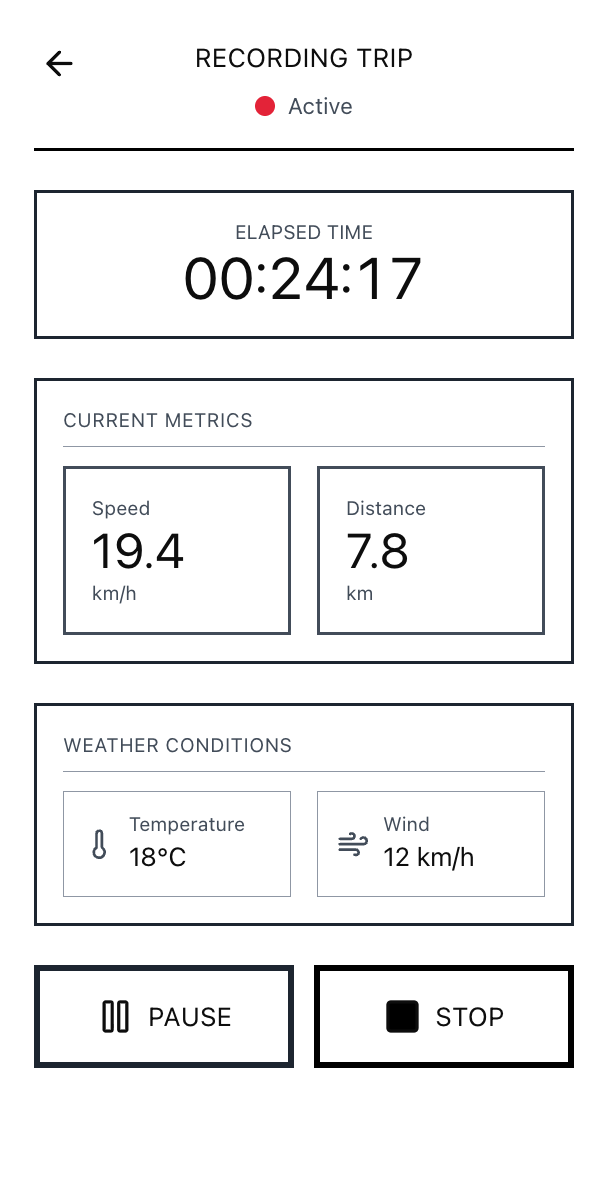
\includegraphics[height=0.8\textheight,keepaspectratio]{mockup_auto_recording.png}

        \column{0.33\textwidth}
        \centering
        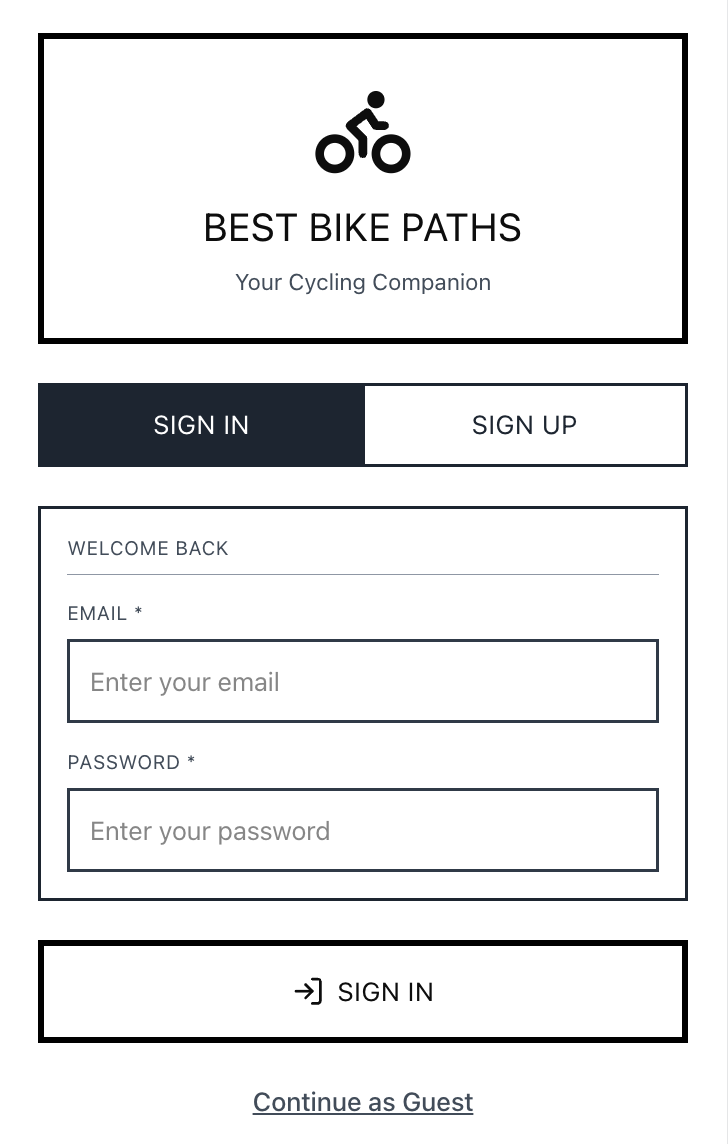
\includegraphics[height=0.8\textheight,keepaspectratio]{signin.png}

        \column{0.33\textwidth}
        \centering
        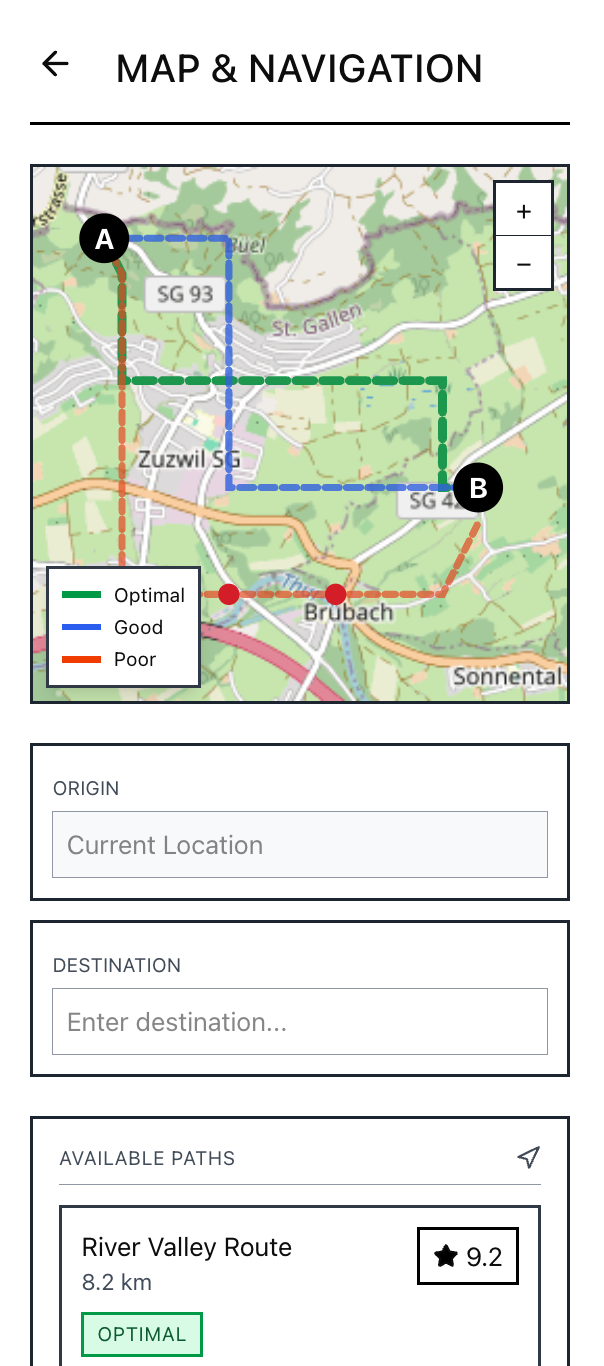
\includegraphics[height=0.8\textheight,keepaspectratio]{mockup_search.png}
    \end{columns}
\end{frame}




% SLIDE 12: Implementation Strategy
\begin{frame}{12. Implementation \& Testing Strategy}
    \textbf{Bottom-Up Approach:}
    
    \vspace{0.3cm}
    \begin{columns}[T]
        \column{0.48\textwidth}
        \begin{enumerate}
            \item \textbf{Step 0:} Data Access Layer \& External Adapters
            \item \textbf{Step 1:} Core Authentication \& User Management
            \item \textbf{Step 2:} Core Algorithms (Scoring, Detection)
            \item \textbf{Step 3:} Service Integration (Ingestion, Reports)
            \item \textbf{Step 4:} Search \& Visualization Layer
            \item \textbf{Step 5:} Client Application Integration
        \end{enumerate}
        
        \column{0.48\textwidth}
        \begin{block}{Testing Strategy}
            \begin{itemize}
                \item \textbf{Unit:} Test drivers for sensor modules
                \item \textbf{Integration:} Service-to-service communication
                \item \textbf{Performance:} 50k concurrent users simulation
                \item \textbf{Security:} GDPR compliance verification
                \item \textbf{Failure:} Offline/crash recovery testing
                \item \textbf{UAT:} Real cyclists with realistic tasks
            \end{itemize}
        \end{block}
    \end{columns}
    
    \vspace{0.3cm}
    \textbf{Mapping to Components:} Each step builds on tested lower-level modules.
\end{frame}

% SLIDE 13: Requirements Traceability
\begin{frame}{13. Requirements Traceability}
    \textbf{Mapping RASD Requirements to DD Components:}
    
    \vspace{0.3cm}
    \centering
    \begin{tabularx}{0.9\textwidth}{lX}
        \toprule
        \textbf{Requirement} & \textbf{Implementing Component(s)} \\
        \midrule
        R01, R02 (Registration/Login) & Users Account Manager Service \\
        R04, R05, R06 (Trip Recording) & Trip Manager (Mobile) + Trip Ingestion Service \\
        R11, R12, R14 (Obstacle Reporting) & Report Server (Ingestion + Validation) \\
        R15, R18 (Obstacle-Street Association) & Report Validation Service + MapAPI Wrapper \\
        R24 (Score Updates) & Trip Scoring Service \\
        R31 (Weather Data) & WeatherAPI Wrapper \\
        R25, R26 (Path Browsing) & Trip Search Server + Map Manager \\
        R33, R34 (Sensor Handling) & Sensor Manager (Mobile) \\
        \bottomrule
    \end{tabularx}
\end{frame}
% SLIDE 14: Requirements Traceability
\begin{frame}{14. Verification} 
    \vspace{0.3cm}
    \begin{block}{Verification}
        \begin{itemize}
            \item All 35 requirements mapped to architectural components
            \item Critical requirements have dedicated services
            \item Non-functional requirements addressed through patterns
        \end{itemize}
    \end{block}
\end{frame}
% =========================================================
% CONCLUSION
% =========================================================
\section{Conclusion}

    \begin{frame}{Conclusion}
    
    \vspace{0.5cm}
    \centering
    \color{BBPBlue}\Large
    \textbf{Thank you for your attention!}
\end{frame}

\end{document}